\section{Introduction}
%Each section needs a subsection for the small points on top to show up
\subsection{Dummy}

\begin{frame}{Quasicrystals}
\(
	\<{6cm}
		\centering
		\includegraphics[scale=0.28]{img/1_intro/homgzn.png}
		
		\ss{3D HoMgZn quasicrystalline sample} \ss{(\url{doi:10.1038/nmat1244})}
	\>
	\<{6cm}
		\centering
		\includegraphics[scale=0.22]{img/1_intro/wasio.jpg}
		
		\ss{A 2D molecular quasicrystal} \ss{(\url{doi:10.1038/nature12993})}
	\>
\)

\begin{itemize}
	\item \ss{Fractal dimensions of wave functions and local spectral measures on the Fibonacci chain}\\\emph{Macé, Jagannathan, Piéchon, PRB 93 (20), 2016}
	\item \ss{Critical eigenstates and their properties in one-and two-dimensional quasicrystals}\\
	\emph{Macé, Jagannathan, Kalugin, Mosseri, Piéchon, PRB 96 (4), 2017}
\end{itemize}
\end{frame}

\begin{frame}{A quasiperiodic puzzle [Bédaride \etal{} 12]}

\centering
\includegraphics[width=.4\textwidth]{img/1_intro/tiles_euro.pdf}

Pay the squares, get the rhombuses for free!

\(
\<{6cm}
\centering
\includegraphics[width=.8\textwidth]{img/1_intro/forbidden.pdf}

Forbidden configuration.
\>

\<{6cm}
\centering
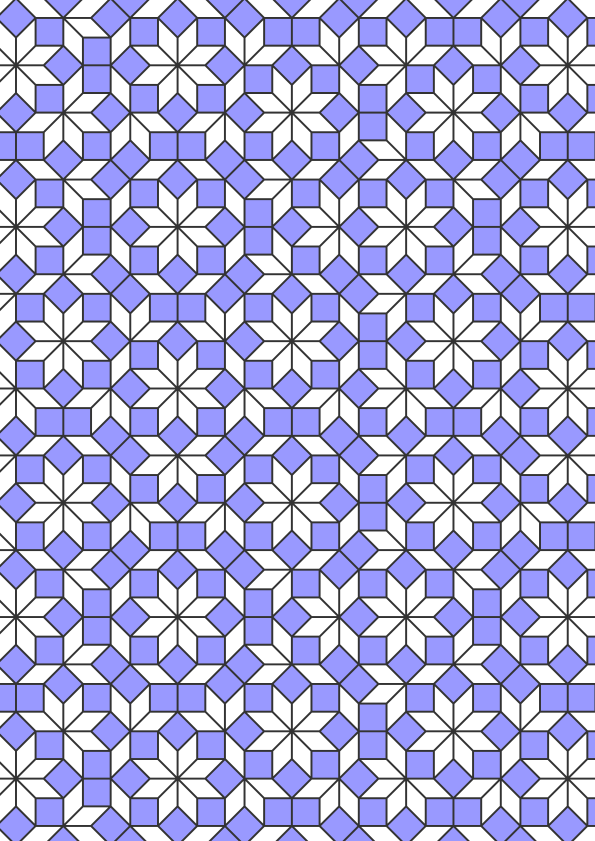
\includegraphics[width=1.\textwidth]{img/1_intro/ammann.pdf}

Patch of the Ammann-Beenker tiling.
\>
\)
\end{frame}

\begin{frame}{Periodic, quasiperiodic and random}
\only<1>{
A random tiling:

\centering
\includegraphics[width=.4\textwidth]{img/1_intro/random00.pdf}

}

\only<2>{
Two copies of the tiling:

\centering
\includegraphics[width=.75\textwidth]{img/1_intro/random01.pdf}

}

\only<3>{
\centering
\includegraphics[width=.6\textwidth]{img/1_intro/random.pdf}

$\to$ no overlap $\to$ no order}

\centering
\only<4>{
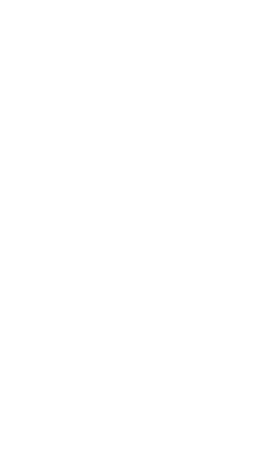
\includegraphics[width=.6\textwidth]{img/1_intro/periodic.pdf}

Perfect long range order: periodic}

\only<5>{
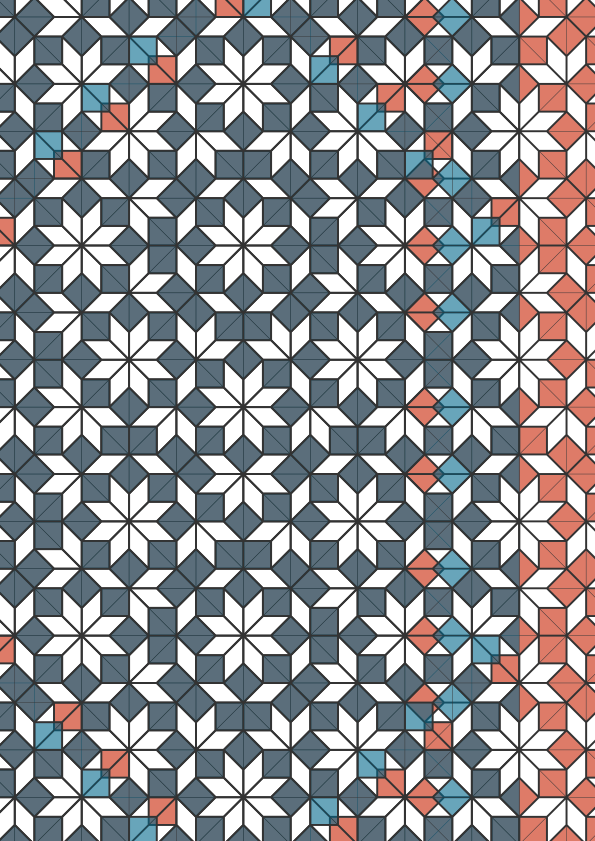
\includegraphics[width=.6\textwidth]{img/1_intro/quasiperiodic.pdf}

Long range order: quasiperiodic 

\flushleft{(see Chap.\ 2 of [Grimm, Baake 13])}
}

\end{frame}

%\begin{frame}{From tiles to atoms}
%Place atoms at the vertices of the tiling:
%
%{\centering
%\includegraphics[width=.6\textwidth]{img/1_intro/AB_tiling_and_plot.pdf}
%
%}
%
%$\rightarrow$ can atoms arrange in such a quasiperiodic fashion?
%\end{frame}

\begin{frame}{Quasicrystals}
Quasicrystal $\to$ quasiperiodically arranged atoms:
\begin{itemize}
	\item \textbf{aperiodicity}
	\item \textbf{long range order} (diffraction pattern exhibits sharp peaks).
\end{itemize}
\(
	\<{6cm}
		\centering
		\includegraphics[scale=0.1]{img/1_intro/diffraction_tenfold.png}
		
		\ss{Diffraction pattern of a AlPdMn alloy} \ss{(Conradin Beeli group)}
	\>
	\<{6cm}
		\centering
		\includegraphics[scale=0.06]{img/1_intro/penrose.png}
		
		\ss{A patch of the quasiperiodic Penrose tiling,} \ss{used to model many quasicrystals.}
	\>
\)
\end{frame}

\begin{frame}{Engineered quasiperiodic structures}
\centering
\includegraphics[width=.5\textwidth]{img/1_intro/dielectric_resonators.png}

{\ss{A network of dielectric resonators [Vignolo \etal{} 14]}}

\begin{itemize}
	\item Plasmons in semiconductor stacks [Merlin \etal{} 85]
	\item Microwaves in perforated metallic films [Matsui \etal{} 07]
	\item Microwaves in dielectric resonator networks [Vignolo \etal{} 14]
	\item Light solitons [Freedman \etal{} 07]
	\item Cold atoms in laser potentials [Guidoni \etal{} 97]
	\item Polaritons in wire cavities [Tanese \etal{} 14]
\end{itemize}
\end{frame}


\begin{frame}{Fractals}
Fractal: object invariant under rescaling
\(
\<{7cm}
\centering
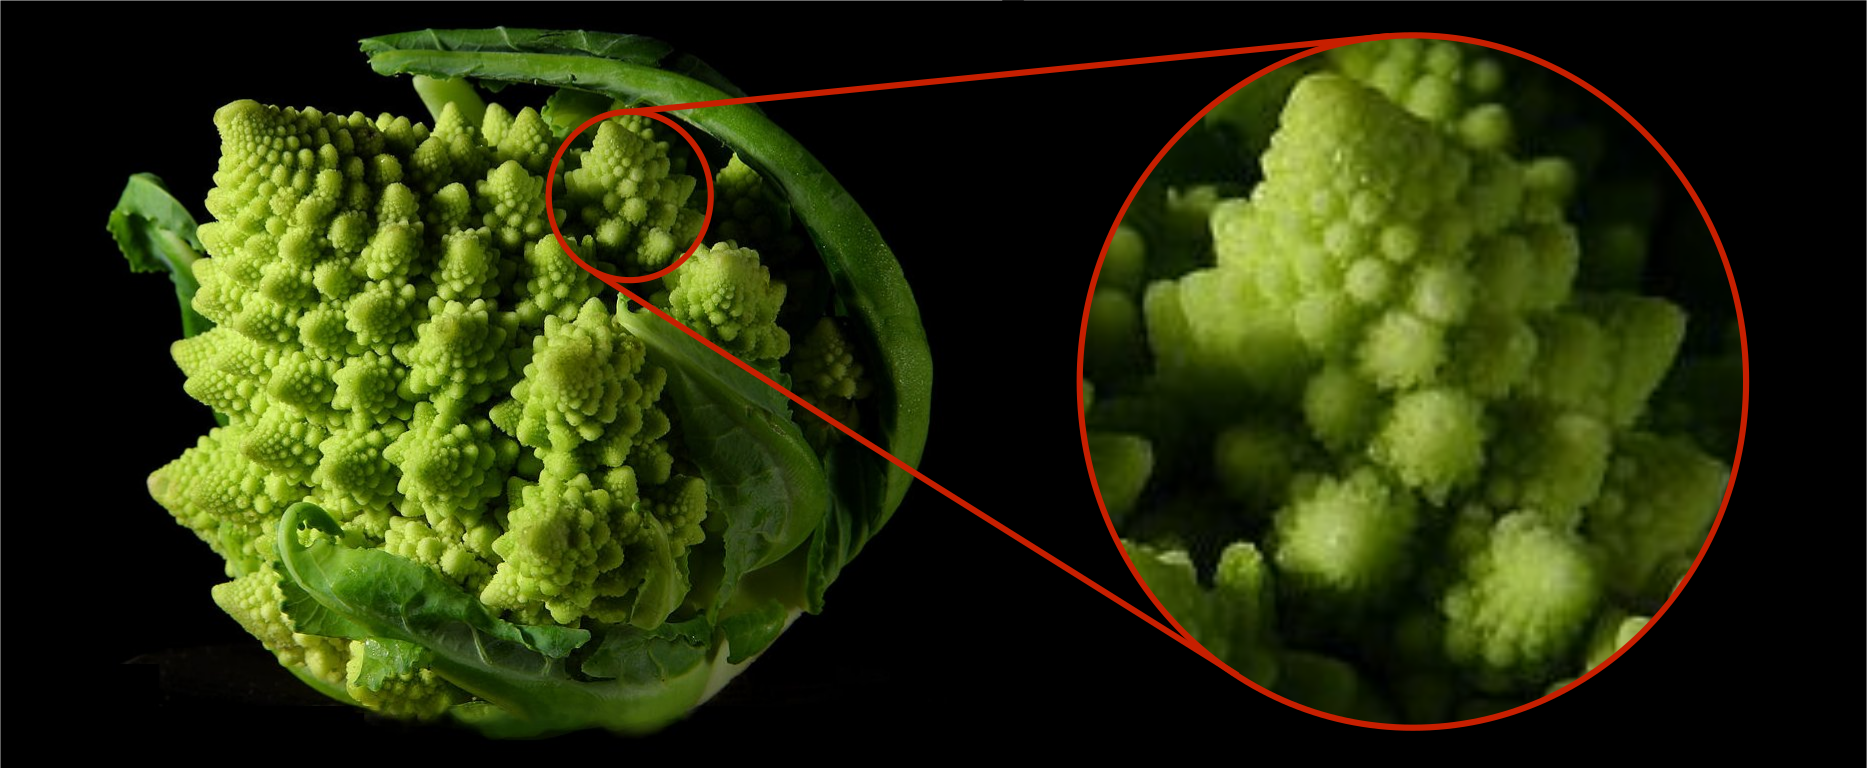
\includegraphics[width=1.\textwidth]{img/1_intro/Fractal_Broccoli.png}

{\ss Romanesco broccoli (\copyleft{} Wikimedia commons)}
\>
\<{7cm}
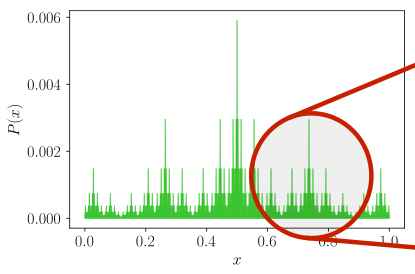
\includegraphics[width=1.\textwidth]{img/1_intro/heights.pdf}

{\ss Electronic density along a quasiperiodic chain}
\>
\)

Quasicrystals \emph{not} fractal\dots

\dots but electrons on quasicrystals $\to$ fractal behavior

\begin{beamerboxesrounded}%
        [shadow=true]%
        {Goal:}
\textbf{Link the fractal behavior of the electrons to quasiperiodicity}
\end{beamerboxesrounded}
\end{frame}